\section{Supporting Measurements for the Main Figures}
\label{app:nine_panel_support}


\paragraph{Teacher-update controls.}
Figure~\ref{fig:subnetwork_overview}(a) compares cumulative parameter changes at update 500 under DR, with additional I64-DT/GT rows; paired points distinguish FP32 and BF16 for each statistic. Panels (b,c) start from the same M-PG/500 student parameters and Adam moments. With domain-specific inputs, each teacher scores responses from its own domain; with shared inputs, all teachers score the same prefixes. Each of four cached response batches contains six teacher pairs. Small points summarize pairs within a batch, and large points average batches. Equation~\ref{eq:history_subtracted} subtracts the Adam step with the current gradient set to zero before computing FP32 update cosines. The resulting step difference remains conditional on the saved moments through Adam's nonlinear update. SGD and reset-$m$ steps are individually rescaled to the norm of the Adam step with trained moments; reset-$m$ retains the second moment and step counter. Teacher pairs reuse teachers and responses, so pairwise observations are dependent. These calculations use non-fused PyTorch updates on copies of saved checkpoints; the online training optimizer uses a fused implementation, allowing numerical differences between them. Mathematics-only and joint training also differ in mathematics prompt exposure (Appendix~\ref{app:setup}).

\paragraph{Vocabulary-supervision controls.}
Figure~\ref{fig:supervision_overview}(a,b) uses four cached response batches at each of four student checkpoints: M-PG and M-I64-DR at updates 100 and 500. Losses use identical prefixes and Adam moments within each checkpoint, while responses can differ between checkpoints. Panel (a) reports batch means. In panel (b), points are individual batches, lines connect PG batch means, and shading spans the I64 measurements. The direction measurements cover PG, I64, and full-vocabulary supervision; I16 appears in the end-to-end training results. Panel (c) compares S-I64, M-I64, and M-I16 with PG at the same task, teacher setting, and update. Table~\ref{tab:local_concentration} adds FP32 and energy-concentration measurements for the M-PG/100 comparison in Appendix~\ref{app:losses}.

\subsection{Additional optimizer and sampling controls}
\label{app:added_controls}

Figure~\ref{fig:normalization_interventions} uses the six cached response batches and training clipping records described in Appendix~\ref{app:fixed_batch_normalization}. In panel (a), boxes mark the interquartile range and whiskers the 5th--95th percentiles; labels give the fraction of training updates clipped. Reset-$m$ and reset-$(m,v)$ retain the optimizer step counter. Panel (c) averages four domain probe losses within each batch; error bars show sample standard deviations over the three batches at each checkpoint.

Figure~\ref{fig:sampling_history_controls}(a) uses three M-PG/100 response batches, with a 4,096-token response cap, containing 48 responses and 288 prefixes. Twelve fixed subsets of prefixes each receive two independent draws of 1, 16, or 64 PG actions per prefix. I64 is evaluated once per subset. Increasing the sample count raises the mean PG gradient cosine to full-vocabulary KL from 0.5374 to 0.8652 and 0.9667; I64 reaches 0.999988. These repeats measure sampling variation at a fixed checkpoint. Panels (b,c) use the separate two-batch experiment with a 256-token response cap (Appendix~\ref{app:records}); its zero-gradient control is evaluated once. Reset-$m$ retains the second moment and step counter, whereas fresh Adam resets both moments and the counter. The sampling and moment-reset comparisons each use their own response batches.

\begin{figure}[t]
\centering
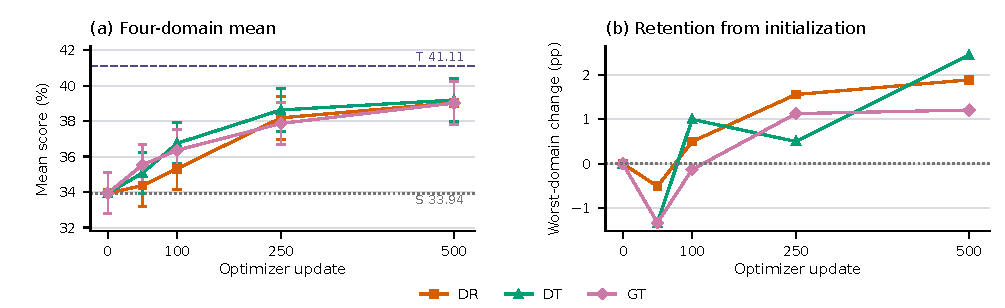
\includegraphics[width=\linewidth]{figures/table1_sync_20260918/section3_capability_support.pdf}
\caption{\textbf{Mean performance gains can coexist with a regression in an individual domain.}
(a) Four-domain mean $\pm$ std; S/T mark the initial student/teacher.
(b) Worst-domain change from initialization; zero means no regression. Lines connect reported point estimates.}
\label{fig:normalization_aggregate_support}
\end{figure}

\paragraph{Cumulative parameter changes.}
Figure~\ref{fig:geometry} shows the trajectories underlying the update-500 summary in Figure~\ref{fig:subnetwork_overview}(a).

\begin{figure}[t]
\centering
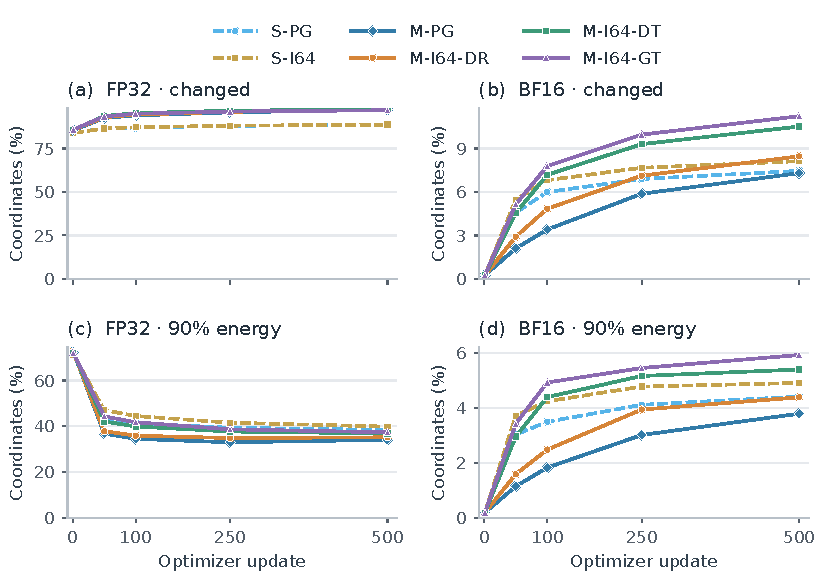
\includegraphics[width=\linewidth]{figures/visual_mvp_20260918/qwen_cumulative_geometry.pdf}
\caption{\textbf{Cumulative BF16 changes remain much sparser than FP32 changes.}
PG/I64 trajectories under DR in single-teacher (S) and joint (M) training, with joint I64-DT/GT added: (a,b) nonzero coordinate fractions; (c,d) coordinate fractions containing 90\% of squared displacement from initialization. Lines connect measured updates 1, 50, 100, 250, and 500; dashed lines denote S. The curves describe the recorded trajectories; uncertainty across training seeds remains unquantified.}
\label{fig:geometry}
\end{figure}

\section{Prompt Exposure and Candidate-Set Weights}
\label{app:recipe_details}

When each domain loss is averaged separately, its prompt quota and loss weight control different quantities. Increasing the quota at fixed $\lambda_d$ changes the number of sampled responses and the variance of the gradient estimate, without directly increasing the domain's expected contribution to the total gradient. Mathematics-only runs receive four times as many mathematics prompts per update as joint runs. Their score differences reflect changes in both teacher count and mathematics exposure.

Candidate-set coverage also scales the distillation gradient. For the student candidate set $S$ and its intersection $I$ with the teacher set in Equation~\ref{eq:topk}, the retained student weights sum to $r(h)=p_\theta(I\mid h)/p_\theta(S\mid h)$. At a fixed prefix with a nonempty intersection and detached coefficients, the I64 gradient equals $r(h)$ times the gradient obtained by renormalizing the same weights over $I$. Coverage therefore changes gradient scale across prefixes even under equal response weighting. Measuring the retained mass and empty-intersection rate by domain can reveal unequal coverage under a fixed candidate size. Enlarging the candidate set or renormalizing its intersection changes the objective and requires a separate performance comparison.
